\documentclass[12pt,a4paper]{article}
\usepackage[top=25.4mm, bottom=25.4mm, left=19.1mm, right=19.1mm]{geometry}


\usepackage[latin2]{inputenc}
\usepackage{graphicx}
\graphicspath{ {./images/} }
\usepackage{ulem}
\usepackage{amsmath}
\usepackage[document]{ragged2e}

\setlength{\parindent}{4em}
\setlength{\parskip}{1em}
\usepackage{hyperref}

\usepackage{fancyhdr}
\pagestyle{fancy}
\fancyhf{}
\fancyhead[LO]{\textbf{\small IoT and Smart Analytics}\\
\text{\small A Program by IIITH and TalentSprint}}

\usepackage{xcolor}
\usepackage{lipsum}

\rhead{\begin{picture}(0,0) \put(-250,-2){
\includegraphics[width=9cm]{EXP_06_Images/ts-iisc-logo-pr.png}} \end{picture}}
\cfoot{\thepage}


\begin{document}

\begin{center}
\textbf{\large \\EXPERIMENT 01 : }Kirchhoff's Laws\\
\textbf{\large \\EXPERIMENT 02 : }Charging/Discharging Phenomenon of a Capacitor
\end{center}

\textbf{\large LEARNING OBJECTIVES:}\\[3pt]
At the end of this experiment, participants will be able to:\vspace{-6mm}\begin{enumerate}
 \setlength\itemsep{-0.3em}
\item verify Kirchhoff's laws
\item understand the charging/discharging phenomenon of a capacitor

\end{enumerate}
\textbf{\large APPARATUS REQUIRED:}\\
\vspace{-3mm}
\begin{enumerate}
 \setlength\itemsep{-0.3em}
\item A Good Internet Connection
\item Digital Multimeter
\item Breadboard
\item Power Adapter
\item DC-DC Voltage Converter Power Supply Module
\item Resistor 1 kilo-ohm (k$\Omega$) - 4pcs
\item Resistor 10 kilo-ohm (k$\Omega$) -2pcs
\item Capacitor 10 microfarad ($\mu$F) -1pcs
\item Jumper Wires
\item Push Buttons-2pcs
\end{enumerate}

\begin{justify}
\textbf{\large A)	Kirchhoff's Law Verification}\\[6pt]
\textbf{\large THEORY}\\[3pt]
Kirchhoff's circuit laws are two equalities that deal with the current and potential difference in the lumped element model of electrical circuits. They are also called Kirchhoff's rules or simply Kirchhoff's laws. These laws can be applied in time and frequency domains and form the basis for network analysis.

\noindent \textbf{Kirchhoff's current law (KCL)}: This law, also called Kirchhoff's second law, states the following: for any node in an electrical circuit, the sum of currents flowing into that node equals the sum of currents flowing out of that node. In other words, the algebraic sum of currents in a network of conductors meeting at a point is zero. It can be written as:  i1 = i2+i3, for the first node moving from left to right in the circuit given in fig.1.

\noindent \textbf{Kirchhoff's voltage law (KVL)}: This law, also called Kirchhoff's second law, states the following: The directed sum of the potential differences around any closed loop is zero. It can be written as: $V_1 + V_2 + V_3 +V_4 = 0$, for the circuit given in fig.2.



\begin{center} 
\includegraphics[scale=0.7]{EXP_1&2_Images/fig1&2.png}
\end{center}
\vspace{-10mm}
\begin{center} {Figure 1. Circuit for KCL \hspace{5cm} Figure 2. Circuit for KVL}\end{center}

\noindent \textbf{\large PROCEDURE}\\[6pt]
\underline{\textbf{Kirchhoff's current law}}\\
The schematic of the circuit is shown in fig.1 above, which we are going to implement. We will add one Multimeter (Amperage mode) in series, with each resistor maintaining the polarity.


\begin{enumerate}
\setlength\itemsep{-0.3em}
\item{\textbf{TinkerCAD}}\\
Dragging and connecting the components: 3 Resistors-each 1k$\Omega$, Power supply-5V, and 3 Multimeters-- as Amperage mode, the final circuit on TinkerCAD looks like as shown in fig. 3 below. After starting the simulation, we can see the result of the current reading and verify the KCL.

\begin{center} 
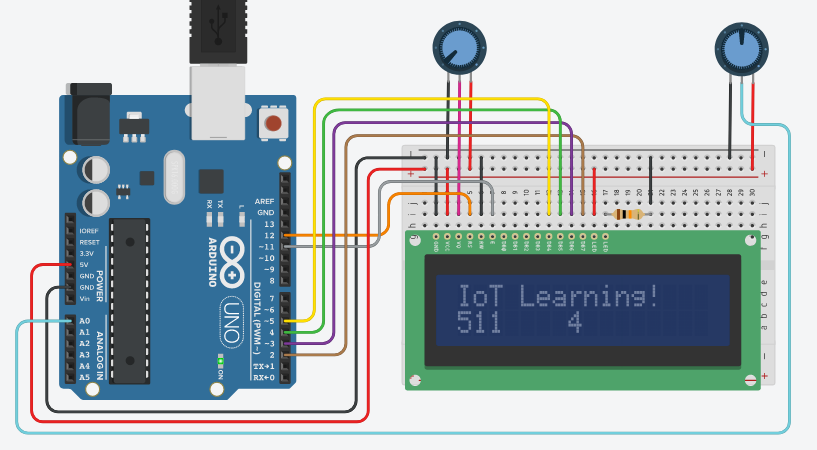
\includegraphics[scale=0.9]{EXP_1&2_Images/fig3.png}
\end{center}
\vspace{-10mm}
\begin{center} {Figure 3. KCL verification on TinkerCAD}\end{center}


\item{\textbf{Physical Realizationa}}

    \begin{enumerate}
    \item Connect 3 resistors of 1 k$\Omega$ on the breadboard as given in fig. 4: two in parallel and the third one in series, as shown in fig. 1 for the circuit diagram.
    \item Connect one end to 5V and the other to GND.
    \item Measure the current going through each resistor (by connecting the Multimeter in series with resistor maintaining the polarity, not shown here) one by one as we have only one Multimeter and verify KCL.
    
    \begin{center} 
    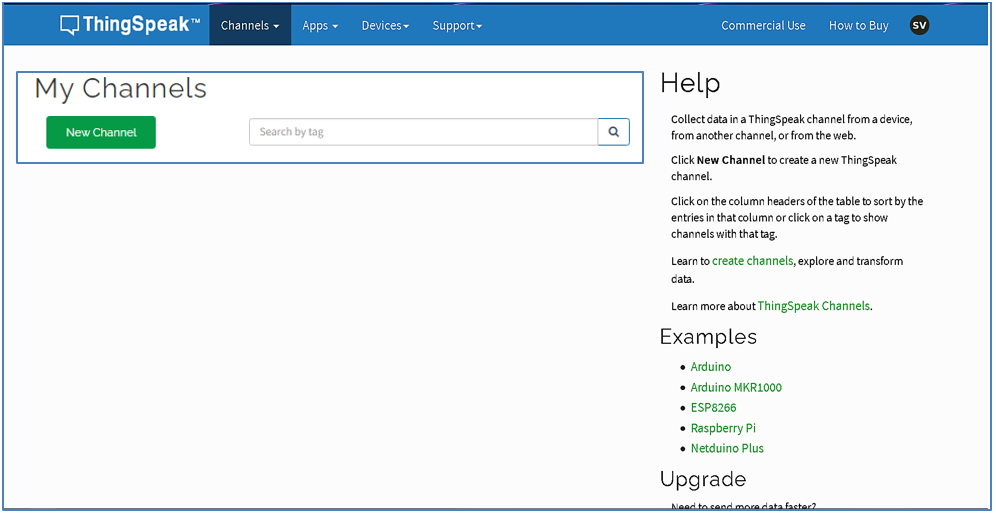
\includegraphics[scale=0.4]{EXP_1&2_Images/fig4.png}
    \end{center}
    \begin{center} {Figure 4. KCL verification with actual hardware}\end{center}
    \end{enumerate}
    
\end {enumerate}

\noindent \underline{\textbf{Kirchhoff's Voltage law }}\\[3pt]
The schematic of the circuit is shown in fig. 5 below, which we are going to implement. We will add one Multimeter (Voltage mode) in parallel with each resistor, maintaining the polarity.

    \begin{center} 
    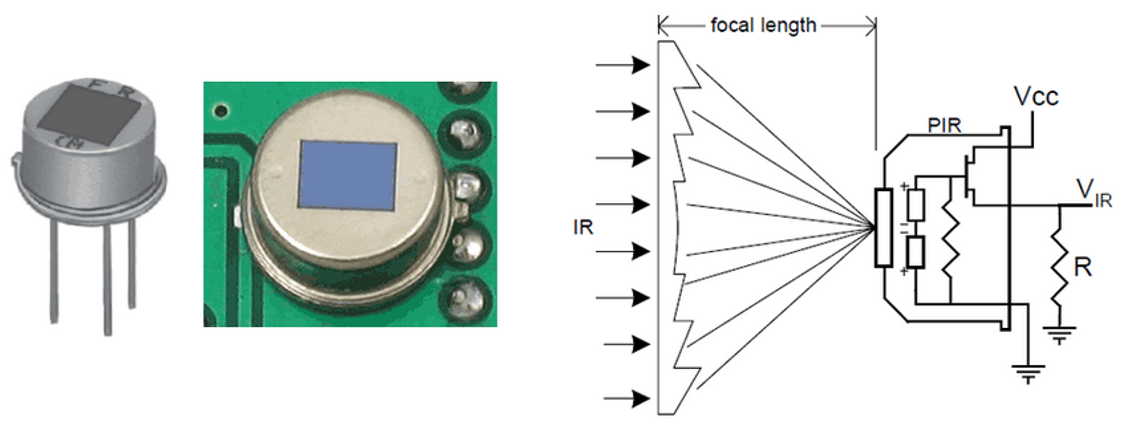
\includegraphics[scale=0.8]{EXP_1&2_Images/fig5.png}
    \end{center}
    \vspace{-5mm}
    \begin{center} {Figure 5. Circuit for KVL}\end{center}

\begin{enumerate}
\item \textbf{TinkerCAD}
    
Dragging and connecting the components: 4 Resistors, each 1k$\Omega$, Power supply- 5V, and 4 Multimeter- selected as voltage mode, the final circuit on TinkerCAD looks like as shown in fig. 6 below. After starting the simulation, we can see the result of voltage reading across each resistor and verify the KVL.


   \begin{center} 
    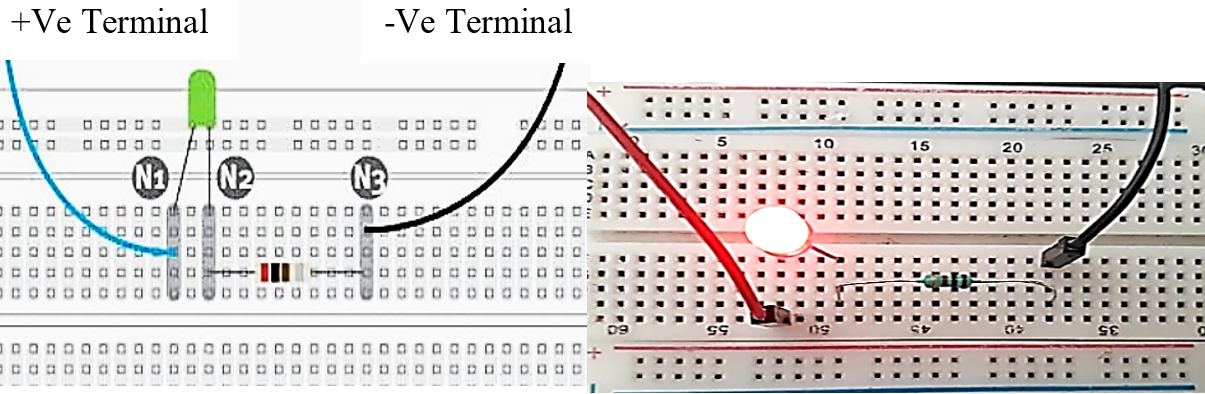
\includegraphics[scale=1]{EXP_1&2_Images/fig6.png}
    \end{center}
    \vspace{-5mm}
    \begin{center} {Figure 6. KVL verification on TinkerCAD}\end{center}
\vspace{2cm}
\item \textbf{Physical Realization\\Hardware Setup}
    \begin{enumerate}
    \item Connect four 1 k$\Omega$ resistors in series with 5V power supply on the breadboard as given in fig. 7; see fig. 5 for the circuit diagram
    \item Measure the voltage across each resistor and verify KVL.
        
    \begin{center} 
    
\includegraphics[scale=0.25]{EXP_1&2_Images/fig7.png}
    \end{center}
    \vspace{-5mm}
    \begin{center} {Figure 7. KVL verification with actual hardware}\end{center}
    \end{enumerate}
    
\end{enumerate}


\noindent \textbf{\large {B) Demonstration of Charging \& Discharging Phenomena of a Capacitor} }\\[6pt]
\textbf{\large THEORY}\\[3pt]
Figure 8 shows a simple RC circuit that employs a dc (direct current) voltage source, a resistor R, a capacitor C, and a switch. The circuit allows the capacitor to be charged or discharged, depending on the position of the switch. When the switch is moved to position A resulting in the circuit in part (b), the capacitor charges. When the switch is moved to position B, the capacitor discharges through the resistor, resulting in the circuit in part (c). Fig. 9 given below shows the charging/discharging voltage curve through a capacitor. 

    \begin{center} 
    
\includegraphics[scale=0.5]{EXP_1&2_Images/fig8.png}
    \end{center}
    \vspace{-5mm}
    \begin{center} {Figure 8. RC circuit with charging \& discharging connections [1]}\end{center}

    \begin{center} 
    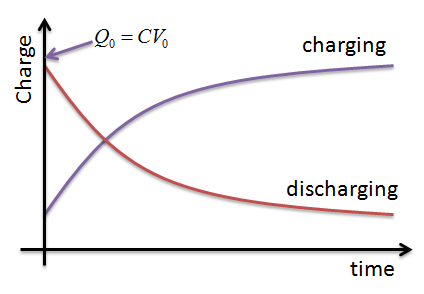
\includegraphics[scale=0.9]{EXP_1&2_Images/fig9.png}
    \end{center}
    \vspace{-5mm}
    \begin{center} {Figure 9. Charging \& discharging curve through a capacitor [2]}\end{center}

\noindent \textbf{\large PROCEDURE}\\[3pt]
The schematic of the circuit is shown in fig.10 below, which we are going to implement. 
    \begin{center} 
    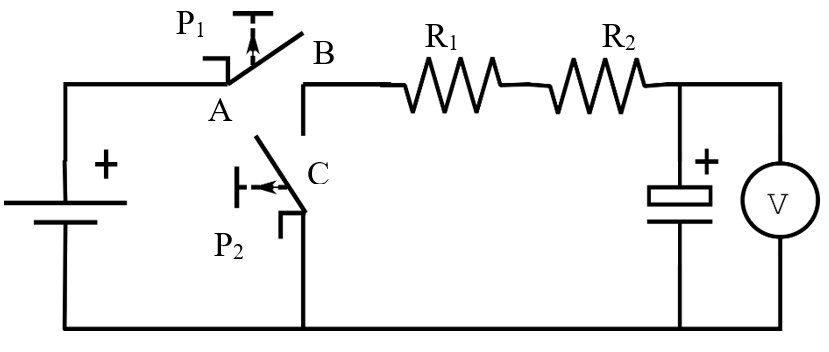
\includegraphics[scale=0.6]{EXP_1&2_Images/fig10.png}
    \end{center}
    \vspace{-5mm}
    \begin{center} {Figure 10.RC circuit for charging and discharging}\end{center}

\begin{enumerate}

\item \textbf{TinkerCAD}\\
Dragging and connecting the components: 2 Resistors-each 10 k$\Omega$, capacitor-10 $\mu$F, Power supply-5V, 2 Pushbuttons, and a Multimeter-selected as voltage mode, the final circuit on TinkerCAD looks like as shown in fig. 11 below. After starting the simulation, when we push the button P1, we will observe a voltage difference b/w the capacitor in Multimeter, fig. 11(a). And when we push the button P2, the voltage starts decreasing, fig. 11(b).

    \begin{center} 
    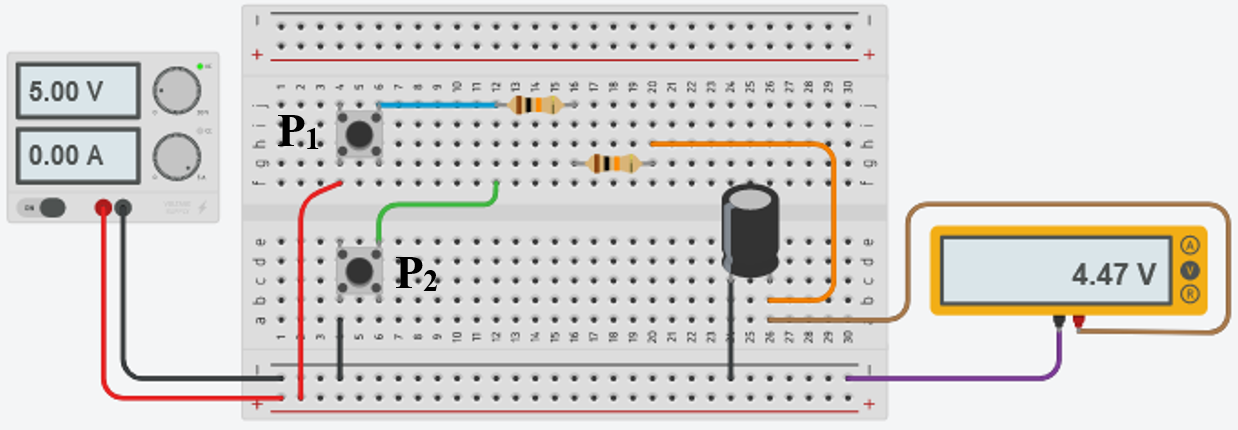
\includegraphics[scale=0.5]{EXP_1&2_Images/fig11a.png}
    \end{center}
    \vspace{-5mm}
    \begin{center} {Figure 11(a). Charging of a capacitor (P1 pushed)}\end{center}
    \begin{center} 
    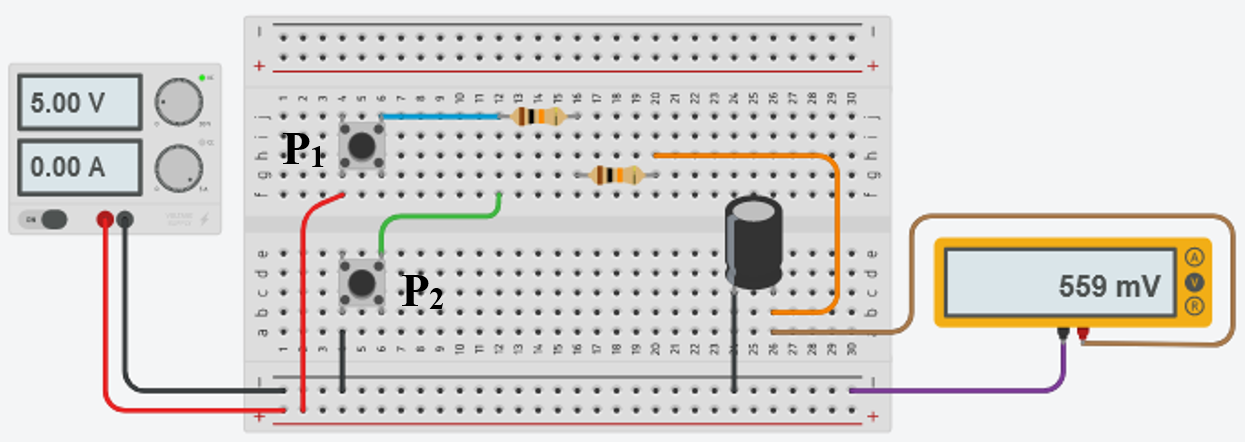
\includegraphics[scale=0.5]{EXP_1&2_Images/fig11b.png}
    \end{center}
    \vspace{-5mm}
    \begin{center} {Figure 11(b). Discharging of a capacitor (P2 pushed)}\end{center}

\item \textbf{Physical Realization}\\[3pt]
For conducting this experiment, we need one 10$\mu$F Capacitor, two 10 k$\Omega$ Resistors, two pushbuttons apart from Multimeter, Power adapter, and DC-DC Voltage Converter.\\[3pt]
\textbf{Safety and Precautions:}
\begin{enumerate}
    \item Always be aware of capacitor polarity before connection.
    \item  Don't touch the charge capacitor.
\end{enumerate}

\textbf{Hardware Setup:}Fig. 12 below shows the hardware setup on a breadboard according to the circuit diagram shown in fig. 10. Instead of a battery, we use a DC-DC converter module as a DC source for the power supply. Follow the steps given below:
\begin{enumerate}
\item Connect the two resistors of 10 k$\Omega$ (R1 and R2) in series and a capacitor of 10$\mu$f on a breadboard.
\item Add a push button P1 with DC source and one pushbutton P2 with a capacitor.
\item Following the circuit diagram in fig. 10, connect the 5V of DC source with R1 through node A of pushbutton P1 and ground to node C of pushbutton P2, connect the remaining end of both push buttons to the end B of R1.
\item Connect Multimeter across the capacitor to measure the voltage (not shown in the figure). When B gets short with A, the capacitor will start charging (Pressing the pushbutton P1) and when B is short with C capacitor starts discharging (Pressing the pushbutton P2). 

    \begin{center} 
    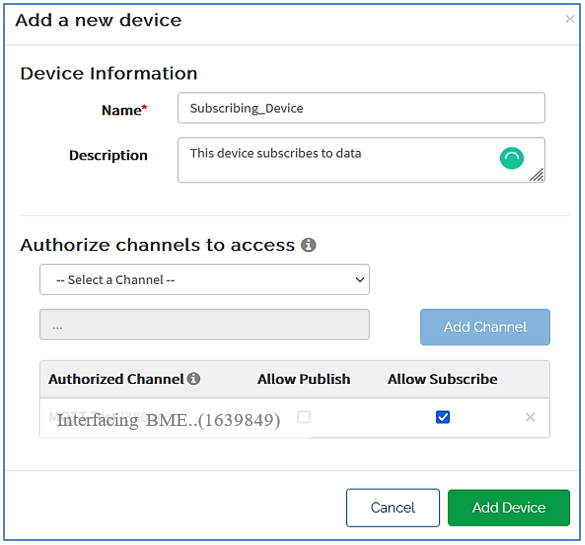
\includegraphics[scale=0.8]{EXP_1&2_Images/fig12.png}
    \end{center}
    \vspace{-5mm}
    \begin{center} {Figure 12. Hardware setup for RC circuit charging/discharging}\end{center}

\end{enumerate}
\end{enumerate}


\setlength{\parindent}{0eM}
\textbf{\large REFERENCES:}
\vspace{-6mm}
\begin{enumerate}
\setlength\itemsep{-0.3em}
 \item  \href{https://opentextbc.ca/universityphysicsv2openstax/chapter/rc-circuits/}{RC Circuits – University Physics Volume 2}
\item   \href{http://www.physbot.co.uk/capacitance.html}{Capacitance}
\item \href{https://en.wikipedia.org/wiki/Kirchhoff%27s_circuit_laws}{Kirchhoff's circuit laws}
\end{enumerate}

\textbf{\large CONCEPT DRILLS:}\\[3pt]
Make a circuit by connecting two Resistors in parallel and an LED in series after that. Connect with power supply maintaining the polarity. Measure voltages/current across/in series with the individual LED/Resistor and verify KCL/KVL.


\end{justify}
\end{document}